\documentclass[main.tex]{subfiles}

\begin{document}
\section{Performance Results Without a framework} \label{sec:prof:cpu}

\subsection{\cpu}

For the \cpu implementation, earlier analysis of the original implementation showed relatively poor scalability. The measured results are not presented here due to different algorithms being employed (since only the PPM version was available at the time for that implementation), and no assumptions could be made about code quality, as explained in \cref{section:impl_original}.
Instead, a scalability analysis was made on the actually implemented \cpu version, shown in \cref{fig:prof:cpu}.

\begin{figure}[!htp]
  \centering
  \begin{subfigure}{.5\textwidth}
    \centering
    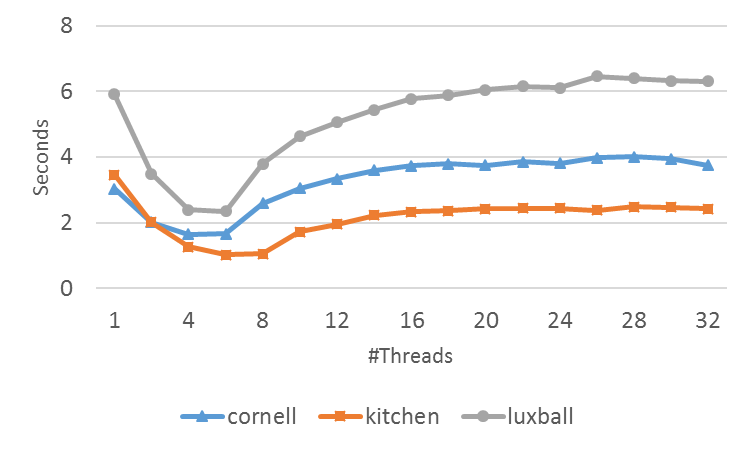
\includegraphics[width=\linewidth]{profiling/cpu_time}
    \caption{Avg iteration time \label{fig:prof:cpu_time}}
  \end{subfigure}%
  \begin{subfigure}{.5\textwidth}
    \centering
    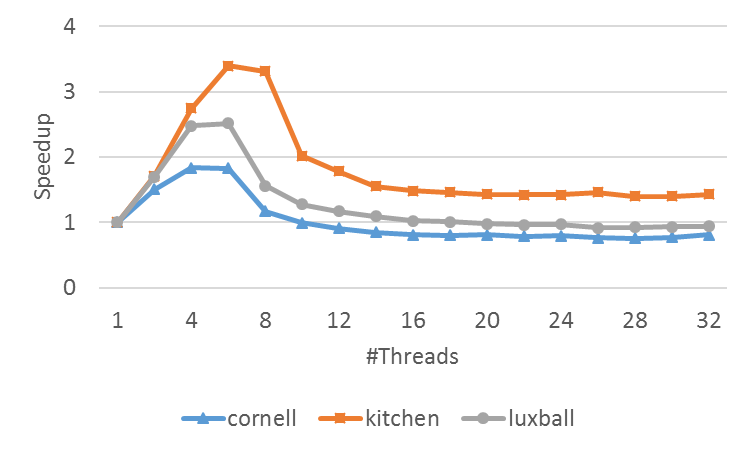
\includegraphics[width=\linewidth]{profiling/cpu_speedup}
    \caption{Speedup \textit{vs} sequential version \label{fig:prof:cpu_speedup}}
  \end{subfigure}
  \caption{\cpu implementation \label{fig:prof:cpu}}
\end{figure}

It can be seen that the code scales fairly up to 6 threads, which is close to the point at which a single \cpu socket is filled, at which point performance starts to degrade.
For \textbf{luxball} and \textbf{cornell} scenes, performance with 16 threads (same amount as physical \cpu cores in the test machine) actually barely differs from the sequential approach.

Scalability is only fair when a single socket is used. The algorithm is clearly memory bounded, especially considering the fact that the test machine uses a \acs{NUMA} architecture. This pins all memory allocated by the master thread (such as the input scene, which is heavily used throughout the algorithm) to one of the sockets, leaving the other with slower access times to such memory.

Memory affinity tools such as \texttt{hwloc} could prove useful here, for example, by creating multiple copies of the input scene, and pinning each one to each \acs{NUMA} node. Each socket would then benefit from faster accesses to its own memory bank.

\subsubsection{\gpu}

When analysing the \gpu implementation, tests were made on both available \gpus, and compared against the base sequential \cpu implementation. The best execution time on \cpu was also included for comparison.

It should be taken into account that, as explained before, this is not a full-\gpu implementation, requiring in-loop memory transfers, and some \cpu computation to generate the lookup table. Since this was not implemented on \gpu, it should add a considerable overhead to the execution. Still, \cref{fig:prof:cuda} shows the implementation is able to outperform the \cpu in two of the three cases, achieving a speedup of around 3 when compared to the sequential approach.

\itodo{proença, sobre o paragrafo acima: convinha relembrar aqui a seq de passos na execução do código, de modo a ficar claro as diversas interacções entre CPU e GPU. Evitar adjectivos}

\begin{figure}[!htp]
  \centering
  \begin{subfigure}{.5\textwidth}
    \centering
    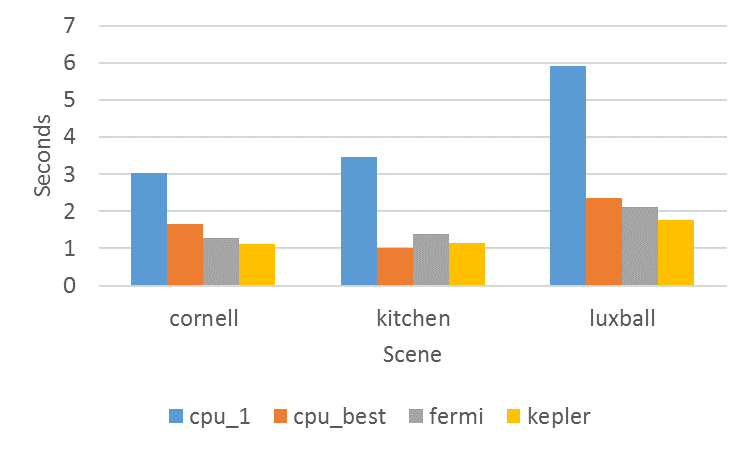
\includegraphics[width=\linewidth]{profiling/gpu_time}
    \caption{Avg iteration time \label{fig:prof:cuda_time}}
  \end{subfigure}%
  \begin{subfigure}{.5\textwidth}
    \centering
    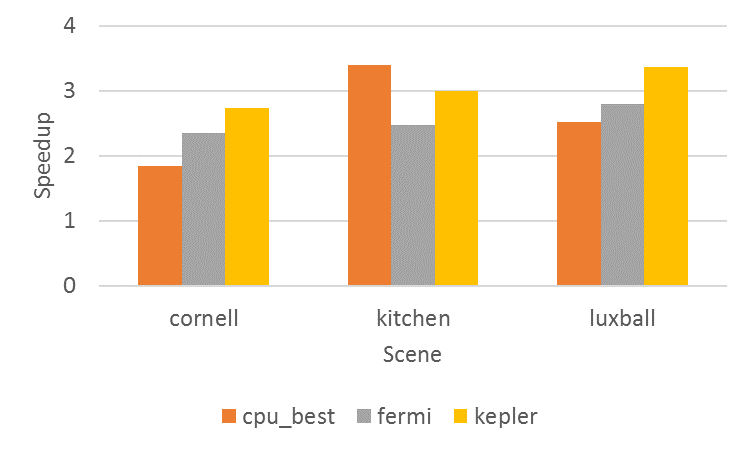
\includegraphics[width=\linewidth]{profiling/gpu_speedup}
    \caption{Speedup vs sequential version \label{fig:prof:cuda_speedup}}
  \end{subfigure}
  \caption{\cuda implementation \label{fig:prof:cuda}}
\end{figure}

\end{document}
